\documentclass[handout]{beamer} %use [handout] mode to ignore overlays (<> commands) 

\usepackage[french]{babel}
\usepackage[T1]{fontenc}
\usepackage[latin1]{inputenc}
\usepackage{soul}

\definecolor{HUGprimary}{RGB}{147,207,169}
\definecolor{HUGsecondary}{RGB}{101,198,193}
\definecolor{HUGtertiary}{RGB}{18,194,242}
\definecolor{HUGtext}{RGB}{18,194,242}

\usetheme{Boadilla}
\setbeamertemplate{footline}[frame number,logo]
\setbeamercolor{structure}{fg=HUGtext}
\usenavigationsymbolstemplate{}
\frenchspacing

\title{DICOM}
\subtitle{Cours HEdS Gen\`eve}
\author[B. Deville]{Beno\^{\i}t Deville~-~Analyste en informatique}
\institute[HUG]{H\^opitaux Universitaires de Gen\`eve}
\date{Session 2023{-}2024}

\begin{document}

\frame{\titlepage}

% repeat outline at each section
\AtBeginSection[] % Do nothing for \section*
{
      \begin{frame}
         \frametitle{Rappel du plan}
         \tableofcontents[currentsection]
      \end{frame}
}

%\section{Notions pr\'eliminaires}

	\frame
	{
		\frametitle{Pour vous, DICOM c'est quoi?}
		%Lien Mentimeter

		\begin{center}
			\includegraphics[width=\linewidth]{../figures/menti.png}
		\end{center}
	}

	\frame
	{
		\frametitle{Qu'est-ce que DICOM}
		\begin{itemize}
			\item Medical
			\item<2-> Imaging
			\item<3-> Standardization
		\end{itemize}
		
		\begin{block}<4->{\textbf{D}igital \textbf{I}maging and \textbf{Co}mmunications in \textbf{M}edicine}
			C'est une norme (ISO 12052) d'interop\'erabilt\'e en imagerie m\'edicale
			
			\url{https://www.dicomstandard.org/current}
		\end{block}
	}

%\section{Principes de DICOM}

	\frame
	{
		\frametitle{Traduire le r\'eel en num\'erique}
		\begin{itemize}
			\item Les actions et objets du monde physique sont mod\'elis\'es de sorte \`a pouvoir les d\'ecrire et les faire exister dans le monde informatique.
			\item<2-> DICOM n'est pas la seule m\'ethode en informatique m\'edicale:
		\end{itemize}
		\begin{columns}
			\begin{column}{0.45\textwidth}
				\begin{block}<3->{DICOM}
					\begin{itemize}
						\item<4-> Mod\`eles Entit\'e / Relation: descriptions du monde r\'eel.
						\item<5-> Paire Objet-Service: un objet num\'erique.
					\end{itemize}
				\end{block}
			\end{column}
			\begin{column}{0.45\textwidth}
				\begin{block}<3->{IHE}
					\begin{itemize}
						\item<4-> Acteurs / Transactions.
						\item<6-> N'est pas limit\'e \`a l'imagerie.
						\item<7> Utilise DICOM.
					\end{itemize}
				\end{block}
			\end{column}
		\end{columns}
	}

	\frame
	{
		\frametitle{Exemple IHE: profil Scheduled Workflow (SWF.b)}
		Traduction dans le r\'eel du flux patient/examen en radiologie:
		\begin{center}
			\includegraphics[width=0.8\textwidth]{../figures/SwfB-v4.png}
		\end{center}
	}

	\frame
	{
		\frametitle{Exemple DICOM: DICOM Model of the Real World}
		Traduction des relations des s\'eries d'un examen DICOM:
		\begin{center}
			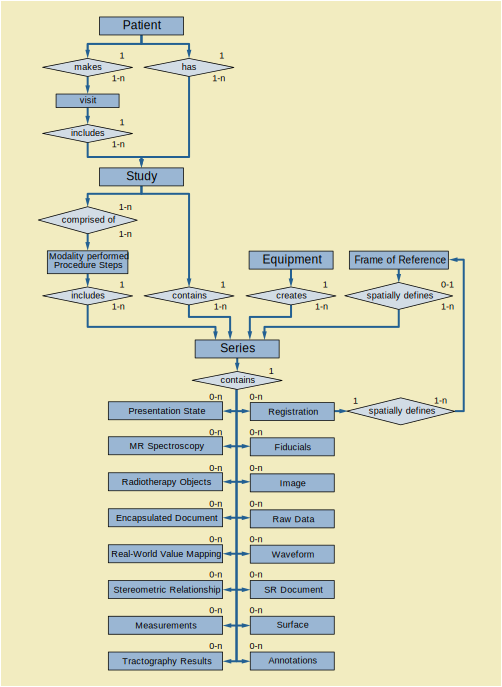
\includegraphics[scale=0.20]{../figures/PS3.png}
		\end{center}
	}

	\frame
	{
		\frametitle{Services principaux}
		\begin{itemize}
			\item Modality Worklist
			\item Store
			\item Modality Performed Procedure Step
			\item Storage Commitment
			\item Query/Retrieve
		\end{itemize}
	}
	
	\frame
	{
		\frametitle{Modality Worklist (MWL)}
		La liste de travail est fournie par le Syst\`eme d'Information Hospitalier (SIH), g\'en\'eralement le RIS.
		
		Son r\^ole et son fonctionnement sont de:
		\begin{itemize}
			\item<2-> assurer l'identitovigilance lors de la r\'ealisation d'un examen sur une modalit\'e,
			\item<3-> permettre la s\'election du protocole \`a effectuer,
			\item<4-> associer de mani\`ere non ambigu\"e les images aux donn\'ees du SIH,
			\item<5-> obtenir du SIH les donn\'ees \`a ajouter obligatoirement dans les images.
		\end{itemize}
		
	}
	
	\frame
	{
		\frametitle{MWL Keys}
			Deux types de \emph{cl\'es} lors de l'interrogation de la worklist:
			\begin{itemize}
				\item<2-> Matching Keys: valeurs sur lesquelles on peut interroger la liste de travail.
				
				On peut vouloir afficher par exemple \emph{Tous les examens du \textbf{jour} pour la modalit\'e nomm\'ee \textbf{RX06}}.
				
				Une matching key est soit \textbf{R}equise, soit \textbf{O}ptionnelle.
				\item<3-> Return Keys: valeurs renvoy\'ees par la liste de travail.
				\begin{description}
					\item<4->[1] Obligatoire.
					\item<5->[2] Obligatoire~-~peut \^etre vide.
					\item<6->[3] Optionnelle.
					\item<7->[<1/2>C] Conditionnelle.
				\end{description}
			\end{itemize}

        \begin{alertblock}<8->{Attention!}
            IHE ajoute des exigences suppl\'ementaires, d\'ecrites dans les profils d'int\'egration.
        \end{alertblock}
	}
	
	\frame
	{
		\frametitle{Modality Performed Procedure Step (MPPS)}
		Le MPPS permet de suivre le statut d'un examen au cours de sa r\'ealisation.

        En fournissant des informations pr\'ecises et \`a jour, ce service est utile pour la facturation, le monitoring par le prescripteur, le workflow du service producteur, le suivi des patients.

		Il peut \^etre 
		\begin{itemize}
			\item<2-> In Progress
			\item<3-> Completed
			\item<4-> Discontinued
		\end{itemize}
	}
	
	\frame
	{
		\frametitle{MPPS In Progress}
		\begin{itemize}
			\item Timing non d\'efini: peut \^etre envoy\'e au d\'ebut comme \`a la fin de la proc\'edure.
			\item<2-> Attributs de tra\c cabilit\'e: normalement issus de la worklist (Scheduled Procedure Step ID, Study Instance UID, Accession Number, d\'emographie patient, \ldots).
			\item<3-> Peut transmettre des d\'etails sur la progression: donn\'ees produites, code des protocoles utilis\'es.
			\item<4-> Notification implicite: un attribut de tra\c cabilit\'e inconnu du SIH peut signifier un examen non programm\'e.
		\end{itemize}
	}
	
	\frame
	{
		\frametitle{MPPS Completed}
		\begin{itemize}
			\item Pas obligatoirement transmis d\`es la fin de la proc\'edure.
			\item<2-> Inclut aussi les attributs de tra\c cabilit\'e.
			\item<3-> Liste
			\begin{itemize}
				\item<4-> les images (et/ou objets) produites (une s\'erie ne peut \^etre r\'epartie entre plusieurs MPPS),
				\item<5-> les protocoles r\'ealis\'es (peuvent diff\'erer de ce qui a \'et\'e planifi\'e),
				\item<6-> le mat\'eriel utilis\'e.
			\end{itemize}
			\item<7-> Peut \^etre compl\'et\'e \emph{a posteriori} par d'autres MPPS.
		\end{itemize}
	}
		
	\frame
	{
		\frametitle{MPPS Discontinued}
		\begin{itemize}
			\item Peut signifer un examen annul\'e ou stopp\'e en cours de route.
			\item<2-> Indique la cause de l'arr\^et.
			\item<3-> Inclut aussi les attributs de tra\c cabilit\'e.
			\item<4-> Peut lister:
			\begin{itemize}
				\item<5-> les images et/ou objets produits,
				\item<6-> les codes des protocoles compl\'et\'es,
				\item<7-> le mat\'eriel utilis\'e.
			\end{itemize}			
		\end{itemize}
	}
	
	\frame
	{
		\frametitle{Attributs}
		\begin{itemize}
			\item Un attribut (\emph{Data Element}) contient une valeur (qui peut \^etre une s\'equence de Data Elements).
			Il est d\'efini par
			\begin{itemize}
				\item<2-> une \'etiquette d'identification (\emph{Tag}) form\'ee de deux valeurs sur 4 chiffres,
				\item<3-> un type (\emph{VR} = \emph{Value Representation}),
				\item<4-> et un nom intelligible.
			\end{itemize}
		
			\item<5-> Exemple: (0020,000D)~---~UI~---~Study Instance UID
			\item<6-> Une image est un Data Element comme un autre, par exemple: (7FE0,0010)~---~OB~or~OW~---~Pixel Data
		\end{itemize}
	}
		
	\frame
	{
		\frametitle{Value Representation}
		DICOM d\'ecrit l'ensemble des types de donn\'ees qu'on peut utiliser dans un fichier: voir le tableau 6.2{-}1 \emph{DICOM Value Representation} du chapitre 5, \emph{Data Structures and Encoding} du standard (\url{http://dicom.nema.org/medical/dicom/current/output/chtml/part05/sect_6.2.html}).
		
		Quelques exemples:
    	\begin{description}
            \item<2->[AS] Age String (e.g. 023Y, 005M, 012D).
            \item<3->[DA] Date, au format YYYYMMDD.
            \item<4->[DT] Date Time, YYYYMMDDHHMMSS.FFFFFF\&{}ZZXX.
            \item<5->[OD] Other Double String (suite de $2^{32}$ octets maximum)
            \item<6->[PN] Person Name (e.g. Doe\^{}John).
		\end{description}
	}

	\frame
	{
		\frametitle{Unique Identifier (UID)}
		\begin{itemize}
			\item Value Representation \textbf{UI}.
			\item<2-> 64 caract\`eres maximum.
			\item<3-> Compos\'es uniquement de chiffres et de points: $\{0-9,.\}$
			\item<4-> Une s\'erie de deux chiffres au moins ne peut commencer par $0$.
			\item<5-> Se divise en deux parties, une \emph{racine} et un \emph{suffixe}: UID~=~\emph{racine}.\emph{suffixe}
			\item<6-> Permet d'identifier de mani\`ere unique un certains nombre d'objets entre diff\'erents pays, sites, vendeurs, et \'equipements.
		\end{itemize}
	}
\frame
{
	\frametitle{Fichier DICOM}
	\begin{itemize}
		\item Single Frame
		\begin{itemize}
			\item Une image: stock\'ee dans un fichier.
			\item Une coupe = une image
		
			$\Rightarrow$ s\'erie de 100 coupes = 100 fichiers.
		\end{itemize}
		\item<2-> Multiframe
		\begin{itemize}
			\item Aussi appel\'e \emph{Enhanced DICOM}.
			\item Plusieurs images dans la m\^eme s\'equence.
			
			E.g. s\'equence vid\'eo d'\'echographie.
		\end{itemize}
		\item<3-> Arborescence des r\'epertoires/fichiers
		\begin{center}
			\includegraphics[width=.8\linewidth]{../figures/arborescence.png}
		\end{center}

	\end{itemize}
}

\frame
{
	\frametitle{Contenu d'un fichier {.dcm}}
	
	Un fichier DICOM est l'agr\'egation des \'el\'ements suivants:
	\begin{itemize}
		\item<2-> Pr\'e-ent\^ete:
		\begin{itemize}
			\item<2-> Pr\'eambule: 128 octets de donn\'ees \emph{application}.
			\item<2-> Pr\'efixe: 0x4449434D=DICM (4 octets).
		\end{itemize}
		\item<3-> Suite de Data Elements:
		\begin{itemize}
			\item<4-> Tag;
			\item<5-> VR;
			\item<6-> Taille;
			\item<7-> et Valeur (qui peut \^etre une s\'equence).
		\end{itemize}
		\item<8-> Et l'image, un Data Element.
	\end{itemize}
}


\frame
{
	\frametitle{Exemple en pratique}
	Exemples avec OsiriX et Weasis.
}

	\frame
	{
		\frametitle{Store}
		Un objet (image, s\'erie, examen, rapport de dose, \ldots) cr\'e\'e par une modalit\'e d'imagerie peut \^etre stock\'ee sur un syst\^eme d'archivage DICOM comme un PACS ou une VNA pour peu qu'il respecte les exigences d'une \emph{Information Object Definition} (IOD).
		\begin{itemize}
			\item<2-> L'IOD d\'efinit les attributs qu'on doit ou peut trouver dans l'objet.
			\item<3-> DICOM divise une IOD en \emph{Information Entities} (IE). Cela permet de d\'efinir des blocs qui seront communs entre diff\'erents types de donn\'ees.
			\item<4-> Une IE est l'association d'un ou plusieurs \emph{Modules}, qui sont
			\begin{description}
				\item<5->[Mandatory] obligatoires,
				\item<6->[Conditional] conditionnels,
				\item<7->[User Option] ou optionnels.
			\end{description}
	   		\item<8-> Les modules indiquent quels attributs peuvent ou doivent \^etre pr\'esents dans l'object \`a stocker
			\begin{description}
				\item<9->[1] Obligatoire.
				\item<9->[2] Obligatoire~-~peut \^etre vide.
				\item<9->[3] Optionnel.
				\item<9->[<1/2>C] Conditionnel.
			\end{description}
		\end{itemize}
	}
	
	% \frame
	% {
 	% 	\frametitle{IOD composite}
	% 	\includegraphics[width=\linewidth]{./figures/IO-composite.png}
	% }

	% \frame
	% {
	% 	\frametitle{Exemple d'IOD : DICOM SR}
	% 	\url{http://dicom.nema.org/medical/dicom/current/output/chtml/part03/sect_A.35.3.3.html}
	% 	\begin{center}
	% 		\includegraphics[width=0.5\linewidth]{./figures/IOD-exemple-SR.png}
	% 	\end{center}
	% }

	\frame
	{
		\frametitle{Exemple d'IOD: image CR}
		\url{http://dicom.nema.org/medical/dicom/current/output/chtml/part03/sect_A.2.3.html}
		\begin{center}
			\includegraphics[width=0.6\linewidth]{../figures/IOD-exemple-CR.png}
		\end{center}
	}

	\frame
	{
		\frametitle{Sch\'ema de l'IOD image CR}
		\begin{center}
			\includegraphics[width=\linewidth]{../figures/IO-definition.png}
		\end{center}
	}
	
    \frame
	{
		\frametitle{Syntaxe de transfert}
		\begin{itemize}
			\item Lorsque la modalit\'e souhaite stocker ses objets, elle doit s'assurer que le syst\`eme cible est capable de comprendre comment les donn\'ees sont repr\'esent\'ees.
			\item<2-> Se met alors en place une n\'egociation entre les deux sys\`emes:
			\begin{enumerate}
				\item<3-> La modalit\'e indique une liste de \emph{presentation contexts} (SOP avec une ou plusieurs syntaxes de tranfert) qu'elle est capable de fournir.
				\item<4-> L'archivage r\'epond en indiquant pour chaque \emph{presentation context} quelle syntaxe de transfert il accepte, ou s'il va tout refuser car il ne supporte aucune des syntaxes propos\'ees.
				\item<5-> La modalit\'e envoie les objets selon la syntaxe n\'egoci\'ee
			\end{enumerate}
			\item<6-> Par souci d'interop\'erabilit\'e, tout syst\^eme de stockage doit supporter au moins une syntaxe de transfert: \emph{Implicit~VR~Little~Endian}.
			\item<7-> Le mieux est \'evidemment quand l'archive peut stocker les objets dans leur format original.
			\item<8-> La liste des syntaxes de transfert se trouve dans le tableau 8.7.3{-}2 de la norme (\url{https://dicom.nema.org/medical/dicom/current/output/chtml/part18/sect_8.7.3.html}).
		\end{itemize}
	}

	\frame
	{
		\frametitle{Storage Commitment}
		\begin{itemize}
			\item Le but de ce service est de s'assurer que les \'el\'ements sont bien stock\'es.
			\item<2-> La modalit\'e fait une requ\^ete au syst\`eme d'archivage (PACS, VNA) avec la liste des UID des objets qui doivent avoir \'et\'e archiv\'es.
			\item<3-> La r\'eponse contient la liste des objets, et en cas d'\'echec, la cause de l'erreur (e.g. probl\`eme de ressources, objets non introuvables,\ldots).
			\item<4-> La modalit\'e peut repousser automatiquement tout objet non stock\'e.
			\item<5-> Peut se faire juste apr\`es le stockage ou de mani\`ere asynchrone (e.g. tous les jours \`a minuit).
			\item<6-> Limitation des risques, d\'emarche qualit\'e.
		\end{itemize}
	}
	
	\frame
	{
		\frametitle{Query/Retrieve}
		\begin{itemize}
			\item Une fois les objets sur l'archivage, d'autres syst\`emes peuvent vouloir y acc\'eder: stations de reconstruction, de navigation, d'interpr\^etation, autres PACS/VNA, etc.
			\item<2-> L'interrogation se fait par crit\`eres \`a diff\'erents niveaux (e.g. patient, examen, s\'erie, image, etc.).
			Ces crit\`eres peuvent se combiner, par exemple:
			\begin{itemize}
				\item<3-> tous les CT du jour,
				\item<4-> les examens des patients dont le nom commencent par DUP effectu\'es le mois dernier.
			\end{itemize}
			\item<5-> Les objets sont ensuite t\'el\'echarg\'es selon ces m\^emes crit\`eres.
		\end{itemize}
	}
    
\frame
{
	\frametitle{Communication}
	\begin{itemize}
		\item Chaque \'equipement joue un r\^ole d\'ependant du service:
		\begin{description}
			\item<2->[SCU] Service Class User (le client).
			\item<3->[SCP] Service Class Provider (le serveur).
		\end{description}
		\item<4-> Le SCU initie une demande, le SCP, qui fournit le service, r\'epond.
	\end{itemize}
	
	\begin{center}
		\includegraphics<5->[width=.8\linewidth]{../figures/scu-scp.png}
	\end{center}
}

\frame
{
	\frametitle{Changement de r\^ole}
	Un \'equipement peut changer de r\^ole.
	
	Par exemple, une station d'interpr\'etation A peut \^etre:
	\begin{itemize}
		\item<2-> SCU dans un premier temps:
		\begin{enumerate}
			\item<3-> A sollicite un examen au PACS;
			\item<4-> Le PACS accepte et envoie l'examen \`a A.
		\end{enumerate}
		\item<5-> puis SCP dans un second temps:
		\begin{enumerate}
		\setcounter{enumi}{2}
			\item<6-> B demande l'examen \`a A;
			\item<7-> A transmet l'examen \`a B.
		\end{enumerate}
	\end{itemize}
	
	\includegraphics<2>[width=.6\linewidth]{../figures/roles-scu.png}
	\includegraphics<3>[width=.6\linewidth]{../figures/roles-1.png}
	\includegraphics<4>[width=.6\linewidth]{../figures/roles-2.png}
	\includegraphics<5>[width=\linewidth]{../figures/roles-scp.png}
	\includegraphics<6>[width=\linewidth]{../figures/roles-3.png}
	\includegraphics<7>[width=\linewidth]{../figures/roles-4.png}
}


\frame
 {
 	\frametitle{Terminologie IHE}
	
	\begin{itemize}
		\item IHE d\'efinit les diff\'erents acteurs et leurs transactions.
		\item<2-> Comme DICOM, IHE indique les champs requis selon les cas, avec sa terminologie propre :	
		\begin{description}
			\item<3->[R] Requis.
			\item<4->[O] Optionnel.
		\end{description}
		\item<5-> Un champs R peut avoir des modificateurs (qui peuvent se combiner) :
		\begin{description}
			\item<6->[R+] 	Exigence suppl\'ementaire par rapport \`a DICOM.
			\item<7->[R*] Attribut requis, mais dont l'affichage n'est pas obligatoire.
		\end{description}
		\item<8-> Un attribut de type 3 dans un IOD, d\'efini comme R dans IHE, doit \^etre consid\'er\'e comme s'il \'etait de type 2.
	\end{itemize}
	
 }

\frame
{
	\frametitle{Et la s\'ecurit\'e dans tout \c ca?}
	\begin{itemize}
		\item DICOM n'a pas \'et\'e con\c cu au d\'epart avec le souci de la s\'ecurit\'e des donn\'ees.
		\item La RGPD est encore r\'ecente.
		\item Les attaques se multiplient et les donn\'ees m\'edicales sont pr\'ecieuses.
		\item Certaines donn\'ees patient sont dans les images.
	\end{itemize}
	Il y a donc des \'evolutions.
	\begin{itemize}
		\item<2-> DICOMweb\texttrademark: profiter de la s\'ecurisation des protocoles Internet pour migrer les services DICOM.
		\item<3-> Outils de d\'esidentification (e,g, Karnak).
	\end{itemize}
}

% \frame
% {
% 	\frametitle{D\'esidentification}
% 	\begin{itemize}
% 		\item Utilisation d'images cliniques pour la recherche ou l'enseignement.
% 		\item<2-> Fichiers mis \`a disposition du public.
% 		\item<3-> N\'ecessit\'e d'anonymat : suppression des informations personnelles permettant d'identifier le patient.
% 		\begin{itemize}
% 			\item<4-> PatientsName (0010,0010)
% 			\item<4-> PatientID (0010,0020)
% 			\item<4-> PatientBirthDate (0010,0030)
			
% 			$\rightarrow$ de type 1 : \`a remplacer, pas supprimer !
% 			\item<4-> ReferringPhysicianName (0008,0090)
% 			\item<4-> etc.
% 			\item<4-> Potentiellement plus de 250 champs \`a supprimer ou \`a vider !
% 		\end{itemize}
% 	\end{itemize}
% }
\frame
{
	\frametitle{Acquisition d'un \'equipement}
	\begin{enumerate}
		\item Avant achat, soumission d'un appel d'offres
		\begin{itemize}
			\item<2-> D\'efinition d'une liste de use cases.

                Exemple: les images brutes export\'ees pourront \^etre r\'eutilis\'ees \emph{a posteriori}.
			\item<3-> R\'edaction du cahier des charges en incluant DICOM et IHE.
			\begin{itemize}
				\item<3-> Pr\'eciser les exigences en termes DICOM et IHE
				
				$\rightarrow$ gr\^ace aux comp\'etences internes,
				
				$\rightarrow$ ou en faisant appel \`a une expertise externe.
				\item<4-> Exiger des documents de conformit\'e DICOM (DICOM Conformance Statement, IHE International Conformity Assessment, r\'esultats Connectathon, etc.).
			\end{itemize}
		\end{itemize}
		\item<5-> Acceptation protocol\'ee
		\begin{itemize}
			\item<6-> V\'erification de la conformit\'e aux profils demand\'es.
			\item<7-> Tests et qualification sur la base des uses cases impliquant
			\begin{itemize}
				\item<8-> le fournisseur,
				\item<9-> le biom\'edical,
				\item<10-> le service informatique,
				\item<11-> les utilisateurs.
			\end{itemize}
		\end{itemize}
	\end{enumerate}
}

\frame
{
	\frametitle{Services \`a demander}
	\begin{center}
		\includegraphics[width=\linewidth]{../figures/tableau-services.png}
	\end{center}
}
\frame
{
	\frametitle{Conclusion}	
	
	\begin{itemize}
		\item Norme incontournable en radiologie.
		\item<2-> Avec DICOM, on est \`a la limite du Plug\&Play dans un SIH bien construit.
		\item<3-> Penser interop\'erabilit\'e \`a long terme.
		\item<4-> Suivre et \'evoluer avec la norme et IHE.
	\end{itemize}
	
	\begin{block}<5->{Ressources}
		\begin{itemize}
			\item Norme DICOM \url{https://www.dicomstandard.org/current}
			\item Innolitics \url{https://dicom.innolitics.com/}
			\item Profiles IHE \url{https://wiki.ihe.net/index.php/Profiles}
			\item Visionneuse Weasis \url{https://weasis.org/}
			\item Simulateur de worklist \url{https://www.fluxinc.ca/public-test-dicom-modality-worklist/}
		\end{itemize}
	\end{block}
}


\end{document}
